\chapter{Fundamentos teóricos}
\thispagestyle{empty}

\section{Aprendizaje automático}
El aprendizaje automático (\textit{Machine Learning}, ML) \cite{22,23} es una rama de la inteligencia artificial y de las ciencias de la computación centrada en el uso de datos y algoritmos para imitar la forma en la que los humanos aprenden, detectando patrones o regularidades para realizar predicciones.

Existen 3 tipos de aprendizaje dentro del ML:

El \textbf{aprendizaje supervisado} consiste en entrenar un modelo con datos que tienen etiquetas conocidas, lo que indica la categoría a la que pertenece cada dato. Por ejemplo, si los datos de entrada son imágenes de animales, las etiquetas podrían ser \enquote*{perro} o \enquote*{gato}. A partir de estos datos etiquetados, el modelo aprende a predecir la etiqueta de nuevos datos. Es el tipo de aprendizaje más utilizado y los datos vienen ya \enquote*{preparados} para su uso. Es el tipo de aprendizaje que utilizaremos en este TFG.

En el \textbf{aprendizaje no supervisado}, el modelo analiza los datos de entrada sin etiquetas, buscando patrones y estructuras inherentes a los datos. El agrupamiento es una técnica común en este tipo de aprendizaje, ya que identifica posibles grupos dentro de los datos. Este enfoque suele requerir un gran volumen de datos para ser efectivo.

Por otro lado, en el \textbf{aprendizaje por refuerzo}, el modelo aprende a través de recompensas o penalizaciones en función de las acciones que realiza. El objetivo del agente es maximizar las recompensas a largo plazo, lo que lo hace especialmente útil en la enseñanza de estrategias en juegos y otras interacciones dinámicas.

\section{Aprendizaje profundo}

\subsection{Redes neuronales artificiales}
Las redes neuronales artificiales (\textit{Artificial Neural Networks}, ANN) \cite{24, 25, 27} son redes computacionales que intentan, a groso modo, simular el proceso de decisión de las neuronas del sistema nervioso central de animales y humano. Las ANN poseen unidades de procesamiento de información llamadas neuronas, las cuales están conectadas entre sí. La estructura básica de una ANN se compone de (ver Figura \ref{fig4}):
\begin{itemize}
	\item Una capa de entrada, que tendrá tantos \textit{inputs} como características o variables tenga el problema
	\item Una o varias capas ocultas, compuestas por neuronas. El número de capas ocultas define la profundidad de la red neuronal.
	\item Una capa de salida, la cual representa el valor o valores predichos
\end{itemize} 

\begin{figure}[h]
	\centering
	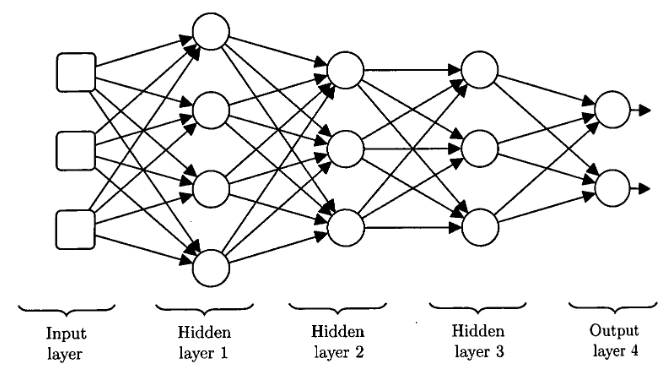
\includegraphics[scale=0.5]{imagenes/cap2/neural-network.png}
	\caption[Esquema de red neuronal.]{Esquema de una red neuronal \cite{26}.}
	\label{fig4}
\end{figure}

Las neuronas son la unidad fundamental de cómputo, tienen varios valores de entrada y un valor de salida que se conecta con las neuronas de la siguiente capa. Los elementos básicos del modelo neuronal son (ver Figura \ref{fig5}):

\begin{itemize}
	\item Un conjunto de conexiones con las señales de entrada. Cada conexión tiene su propio peso/fuerza.
	\item Una función de suma de las señales de entrada, ponderadas cada una con su peso. Estas operaciones constituyen una combinación lineal.
	\item Una función de activación, para limitar la amplitud de la salida de la neurona. Normalmente, el rango de salida está en el intervalo [0,1], o alternativamente en [-1,1]. Existen muchos tipos de funciones de activación pero, se suelen utilizar cuatro: la función signo, la función logística, la función arco-tangente o la función ReLU (\textit{Rectified Linear Unit}).
\end{itemize} 

\begin{figure}[h]
	\centering
	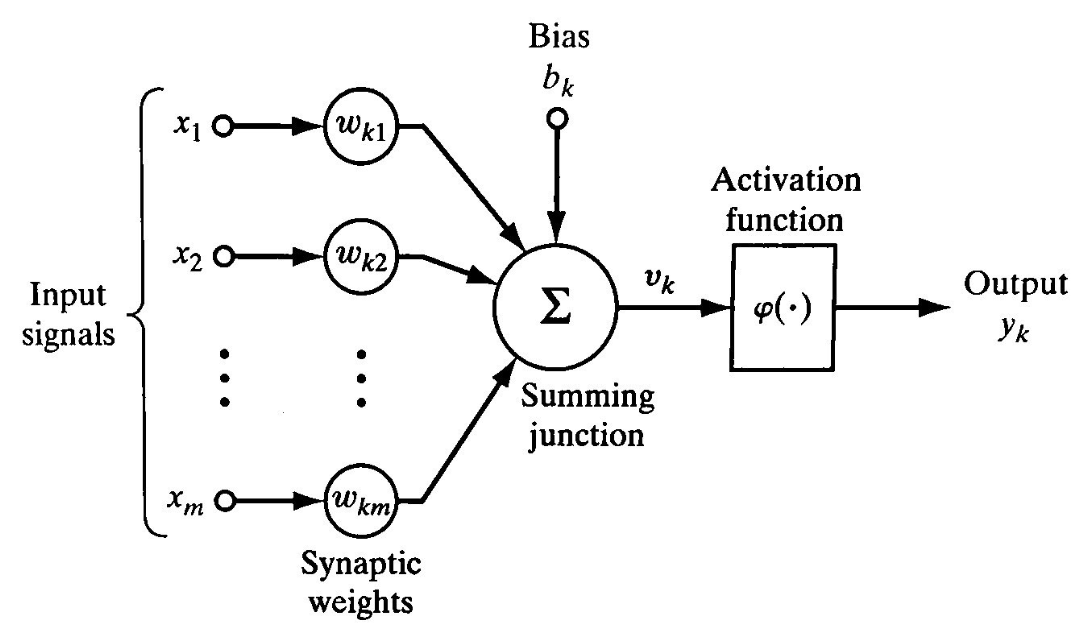
\includegraphics[scale=0.25]{imagenes/cap2/neuron-model.png}
	\caption[Modelo neuronal.]{Modelo neuronal para una neurona $k$ \cite{25}.}
	\label{fig5}
\end{figure}

En términos matemáticos, podemos describir la salida de una neurona como:

\begin{equation}
	y = \phi(\sum_{j=1}^{m} w_j x_j + b)
\end{equation}

siendo $\phi$ la función de activación, $m$ el número de señales de entrada, $w_j$ el peso de cada entrada $x_j$, y $b$ el sesgo.

El algoritmo de aprendizaje de la red neuronal consiste en ir modificando los pesos y el sesgo, iterativamente, hasta alcanzar el resultado deseado. Este proceso iterativo se conoce como entrenamiento, y permite, a través de las modificaciones de los pesos, reconocer y extraer las características más relevantes de los datos.

El objetivo del entrenamiento es minimizar el error de predicción de la salida de la red neuronal, para ello, se define una función de pérdida. Existen numerosas funciones de pérdida, algunas de las más conocidas son: el error cuadrático medio (MSE), el error absoluto medio (MAE) o la entropía cruzada. La información de la función de pérdida se transmite desde la salida a la capa inicial, con el fin de modificar adecuadamente los pesos para generar una mejor estimación de la predicción.

Uno de los aspectos más importantes al entrenar un modelo es el sobreajuste. Este fenómeno ocurre cuando el modelo se adapta excesivamente al conjunto de datos de entrenamiento, lo que resulta en un rendimiento deficiente al enfrentarse a nuevos datos no incluidos en el entrenamiento. Esto se debe a una limitada capacidad de generalización, que puede mitigarse mediante técnicas de regularización \ref{regularizacion}.


\subsection{Redes neuronales convolucionales}
Las redes neuronales convolucionales (\textit{Convolutional Neural Networks}, CNN) \cite{35, 36, 37} son un tipo de red neuronal profunda que trabaja con patrones de cuadrícula, como pueden ser imágenes (ver Figura \ref{fig6}).

En estas redes neuronales, las capas convolucionales desempeñan un papel fundamental, y a menudo se complementan con capas de \textit{pooling}. Dichas capas se encuentran en la primera parte de la red y son las encargadas de extraer las características relevantes de la entrada. Esto posibilita la automatización del proceso de extracción de características, mejorando simultáneamente tanto el tiempo como el rendimiento.

\begin{figure}[h]
	\centering
	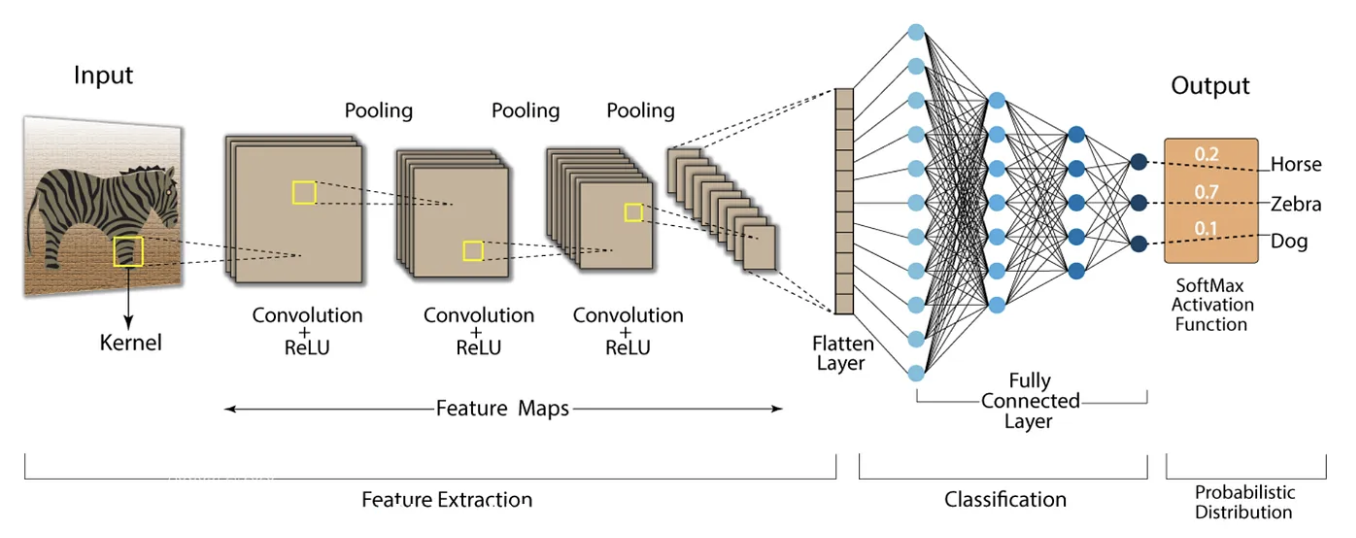
\includegraphics[scale=0.5]{imagenes/cap2/cnn.png}
	\caption[Ejemplo de red neuronal convolucional.]{Ejemplo de red neuronal convolucional \cite{41}.}
	\label{fig6}
\end{figure}

A continuación, se describen los posibles tipos de capas presentes en una CNN \cite{39,40}:


\subsubsection*{Capa de convolución}

La capa convolucional es un componente fundamental de las CNN, utilizada para la extracción de características de una imagen o un conjunto de imágenes. Esta capa aplica una operación lineal especializada conocida como convolución, que consiste en aplicar un filtro o \textit{kernel} a la imagen de entrada. El \textit{kernel} es una matriz que se desliza a lo largo de la imagen, multiplicando sus valores con los píxeles correspondientes y sumándolos para producir un único valor en la imagen de salida. Este proceso se repite en todas las posiciones de la imagen dando como resultado una nueva matriz denominada mapa de características (ver Figura \ref{fig7}).

\begin{figure}[h]
	\centering
	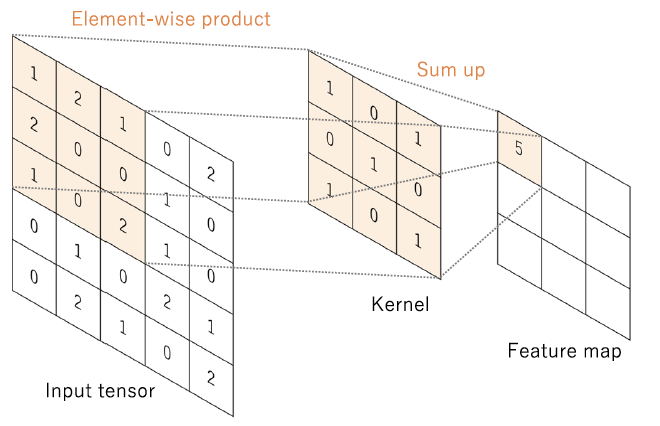
\includegraphics[scale=0.75]{imagenes/cap2/convolution.png}
	\caption[Ejemplo de operación de convolución.]{Ejemplo de operación de convolución en CNN \cite{40}.}
	\label{fig7}
\end{figure}

Los pesos de los filtros se aprenden durante el proceso de entrenamiento de la red neuronal. Cada \textit{kernel} tiene sus propios pesos que se ajustan iterativamente durante el entrenamiento para minimizar la función de pérdida y mejorar el rendimiento del modelo.

La característica clave de la operación de convolución es el \textit{weight sharing}, que implica compartir los mismos \textit{kernels} en toda la imagen. Esto permite que la red detecte patrones locales independientemente de su ubicación en la imagen. Además, contribuye a aprender jerarquías de características espaciales, lo que permite capturar una amplia gama de características en varios niveles de abstracción. Este enfoque también aumenta la eficiencia del modelo al reducir la cantidad de parámetros que necesita aprender en comparación con las redes totalmente conectadas.

Por otro lado, es importante la configuración de los hiperparámetros de cada capa convolucional, estos se definen antes de iniciar el entrenamiento de la red neuronal y afectan al comportamiento de la misma. Los más comunes son:
\begin{itemize}
	\item Tamaño del \textit{kernel}: se refiere a las dimensiones del filtro que se aplica a la imagen de entrada. Los tamaños comunes son 3x3, 5x5 o 7x7.
	\item Número de \textit{kernels}: indica cuántos filtros se aplicarán a la imagen de entrada para extraer diferentes características. Cuantos más \textit{kernels} se utilicen, mayor será la profundidad de los mapas de características de salida.
	\item \textit{Padding}: esta técnica consiste en añadir píxeles alrededor de la imagen de entrada tras el proceso de convolución. Su propósito es mantener el tamaño de la salida, ya que al aplicar la convolución, las dimensiones del mapa de características se reducen con respecto a la imagen original.
	\item \textit{Stride}: es el número de píxeles que se desplaza el \textit{kernel} en cada paso durante la convolución. Un mayor \textit{stride} reduce el tamaño del mapa de características y la cantidad de operaciones necesarias.
\end{itemize}

Sin embargo, es importante tener en cuenta que la operación de convolución por sí sola es lineal y puede no ser suficiente para aprender patrones complejos. En este contexto, entra en juego la capa de activación, que introduce no linealidades en la red y potencia su capacidad para capturar relaciones más complejas entre las características extraídas.

\subsubsection*{Capa de activación}

La capa de activación en una CNN sigue a la capa convolucional y se encarga de introducir no linealidades en el modelo mediante una función de activación.
Esta función aumenta la capacidad de la red para aprender relaciones no lineales en los datos, lo que es fundamental para capturar patrones más complejos. Algunas de las funciones de activación comunes utilizadas son la función ReLU, la función sigmoide y la función tangente hiperbólica (ver Figura \ref{fig8}).

\begin{figure}[h]
	\centering
	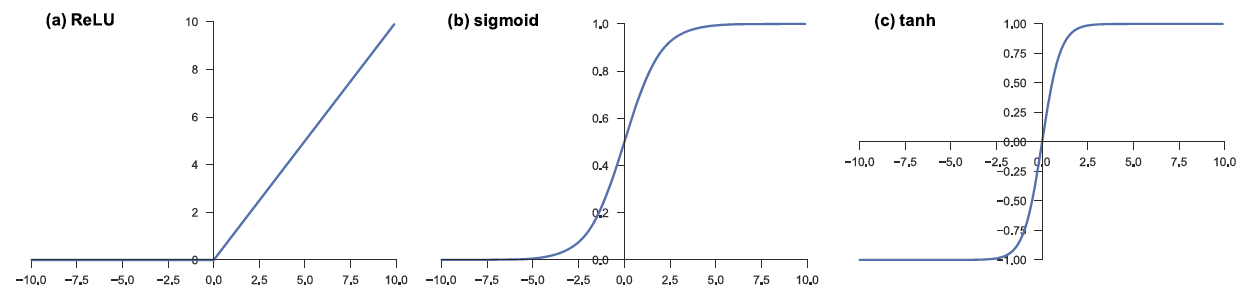
\includegraphics[scale=0.55]{imagenes/cap2/activation.png}
	\caption[Funciones de activación comunes.]{Funciones de activación comúnmente aplicadas en CNN \cite{40}.}
	\label{fig8}
\end{figure}

\subsubsection*{Capa de \textit{pooling}}
La capa de \textit{pooling} también es específica de las CNN y se encarga de reducir la dimensionalidad de las características conservando la información más relevante.

Esta capa resume la información en regiones locales mediante una operación de \textit{downsampling} en las características de entrada. Al reducir la dimensionalidad de las características, la capa de \textit{pooling} disminuye el número de parámetros aprendibles en la red, lo que puede ayudar a prevenir el sobreajuste y mejorar la eficiencia computacional del modelo. Además, esta capa también ayuda a introducir invariancia a pequeñas traslaciones y distorsiones en los datos de entrada, permititiendo a la red reconocer patrones incluso si están ligeramente desplazados en la imagen. 

Los dos tipos más comunes de \textit{pooling} son el \textit{max pooling}, que selecciona el valor máximo de una región local en las características de entrada, y el \textit{average pooling}, que calcula el promedio de los valores en una región local (ver Figura \ref{fig9}).

\begin{figure}[h]
	\centering
	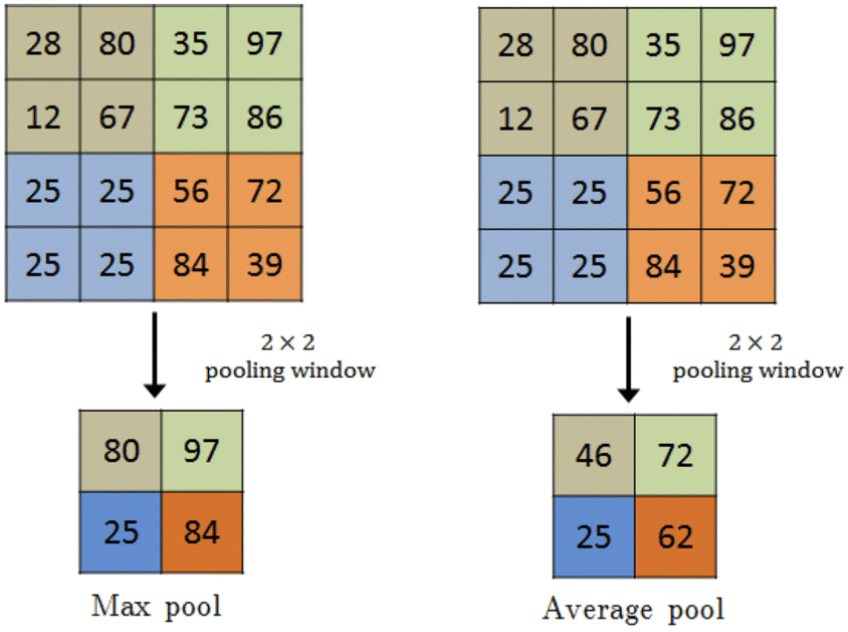
\includegraphics[scale=0.55]{imagenes/cap2/pooling.png}
	\caption[Tipos de \textit{pooling} comunes.]{Tipos de \textit{pooling} comúnmente utilizados en CNN \cite{42}.}
	\label{fig9}
\end{figure}

Los hiperparámetros de la capa de \textit{pooling} incluyen el tamaño del filtro, el \textit{stride} y el tipo de \textit{padding}. Estos hiperparámetros afectan la forma en que se realiza el \textit{downsampling} en las características.

\subsubsection*{Capa totalmente conectada}

La capa totalmente conectada sigue a las capas de convolución y \textit{pooling}. En esta capa, las características extraídas por las capas anteriores se transforman en un formato unidimensional (vector) antes de conectarse a una o más capas totalmente conectadas, también conocidas como capas densas.

Esta capa, al igual que en las redes neuronales clásicas, tiene la responsabilidad de combinar y procesar las características extraídas para producir la salida final de la red.

Cada neurona en una capa totalmente conectada está conectada a todas las neuronas de la capa anterior a través de pesos aprendibles. Estos pesos determinan la contribución de cada neurona de entrada a la neurona de salida correspondiente en la capa totalmente conectada. Durante el entrenamiento, estos pesos se ajustan mediante algoritmos de optimización como \textit{backpropagation} y descenso de gradiente para minimizar la diferencia entre las salidas predichas y las etiquetas reales.

Es importante destacar que la capa totalmente conectada suele estar seguida por una función de activación no lineal, como ReLU, para introducir no linealidades en el modelo y permitir la representación de patrones complejos en los datos. Además, la última capa de activación de la CNN, generalmente se selecciona según la naturaleza de la tarea que se está abordando.

\subsection{Transferencia de aprendizaje}

La transferencia de aprendizaje \cite{49}, también conocida como \textit{Transfer Learning} (TL), es una técnica fundamental en el campo del aprendizaje automático. Consiste en aprovechar el conocimiento adquirido al resolver un problema para mejorar el rendimiento en otro problema relacionado. En lugar de comenzar desde cero al entrenar un modelo para una tarea específica, el TL utiliza el aprendizaje previo en tareas similares, obteniendo múltiples beneficios, como una mayor eficiencia en el entrenamiento de modelos, una mejor generalización con conjuntos de datos limitados y una aceleración en el desarrollo de modelos.

En las arquitecturas convolucionales, la forma más común de llevar a cabo la transferencia de aprendizaje es mediante el \textit{fine-tuning} \cite{39}, que implica utilizar pesos pre-entrenados, congelar todas las capas de la red excepto las superiores, y ajustar estas últimas para adaptarlas a nuestro problema específico, de manera que el entrenamiento se realice únicamente en esas capas superiores. Este enfoque aprovecha la capacidad de los modelos pre-entrenados para capturar características generales de los datos, lo cual es especialmente útil cuando se dispone de conjuntos de datos pequeños o limitados. Además, al congelar las capas iniciales se evita la pérdida de información importante aprendida durante el pre-entrenamiento, mientras que el \textit{fine-tuning} en las capas superiores permite adaptar el modelo a la nueva tarea específica.

En este contexto, es común utilizar los pesos pre-entrenados en el conjunto de datos de ImageNet \cite{50} debido a su gran tamaño, diversidad, representatividad y disponibilidad.


\subsection{Regularización}\label{regularizacion}
Tanto en las redes neuronales clásicas como en las convolucionales, el sobreajuste a los datos de entrenamiento es una problema importante (ver Figura \ref{fig10}). Aunque la solución óptima sería adquirir más datos para el entrenamiento, esta opción no siempre está disponible. Por tanto, se recurre a técnicas de regularización para mitigar este problema. Entre las más destacadas se encuentran:

\begin{itemize}
	\item \textit{Dropout}: es una técnica de regularización donde se establecen aleatoriamente ciertas activaciones a 0 durante el entrenamiento, de modo que el modelo se vuelve menos sensible a pesos específicos en la red.
	\item \textit{Weight decay}: también conocido como regularización L2, reduce el sobreajuste penalizando los pesos del modelo para que tomen solo valores pequeños.
	\item \textit{Batch normalization}: es un tipo de capa suplementaria que normaliza adaptativamente los valores de entrada de la siguiente capa, mitigando el riesgo de sobreajuste, así como mejorando el flujo de gradiente a través de la red, permitiendo tasas de aprendizaje más altas y reduciendo la dependencia de la inicialización.
	\item \textit{Data augmentation}: es un proceso de modificación de los datos de entrenamiento a través de transformaciones aleatorias, como volteo, traslación, recorte, rotación y borrado aleatorio, para que el modelo no vea exactamente las mismas entradas durante las iteraciones de entrenamiento. Esta técnica, además de reducir el sobreajuste, permite una mejor generalización del modelo.
	\item Elección del modelo: un modelo de una alta complejidad puede provocar sobreajuste ya que tiene la capacidad de ajustarse mucho mejor a los datos de entrenamiento. Es fundamental encontrar un modelo que tenga un equilibrio entre complejidad y generalización, es decir, que sea lo suficientemente complejo para captar las características importantes pero que a la vez sea capaz de generalizar sin sobreajustarse demasiado a los datos.
\end{itemize}

\begin{figure}[h]
	\centering
	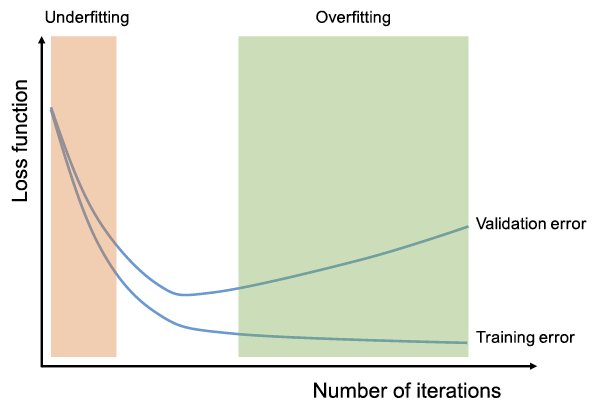
\includegraphics[scale=0.8]{imagenes/cap2/sobreajuste.png}
	\caption[Infraajuste y sobreajuste en entrenamiento.]{Zona de infraajuste y sobreajuste durante el entrenamiento \cite{40}.}
	\label{fig10}
\end{figure}

A pesar de las técnicas anteriores, persiste la preocupación por el sobreajuste al conjunto de validación en lugar del conjunto de entrenamiento, principalmente debido a la filtración de información durante el ajuste fino de hiperparámetros y el proceso de selección del modelo. Por tanto, es importante evaluar el rendimiento del modelo final en un conjunto de prueba separado, preferiblemente no visto previamente. Esto es fundamental para validar la capacidad de generalización del modelo y garantizar su fiabilidad.


\section{Parámetros de la cámara}

A la hora de trabajar con imágenes faciales y, particularmente, para comprender todos los factores que intervienen en el proceso de la simulación de imágenes faciales, es esencial introducir una serie de conceptos relativos a los parámetros de la cámara \cite{51,67,68,69}. Estos parámetros, como la longitud focal, el sensor de la cámara y la distancia cámara-sujeto, entre otros, están estrechamente relacionados entre sí y ejercen una influencia significativa tanto en la configuración de la escena fotográfica como en la percepción visual de los sujetos retratados en ella.

\subsection*{Longitud focal}
La longitud focal mide la distancia, en milímetros, entre el \textit{punto nodal} (punto donde la luz converge en una lente) y el sensor de la cámara (ver Figura \ref{fig11}). 

\begin{figure}[h]
	\centering
	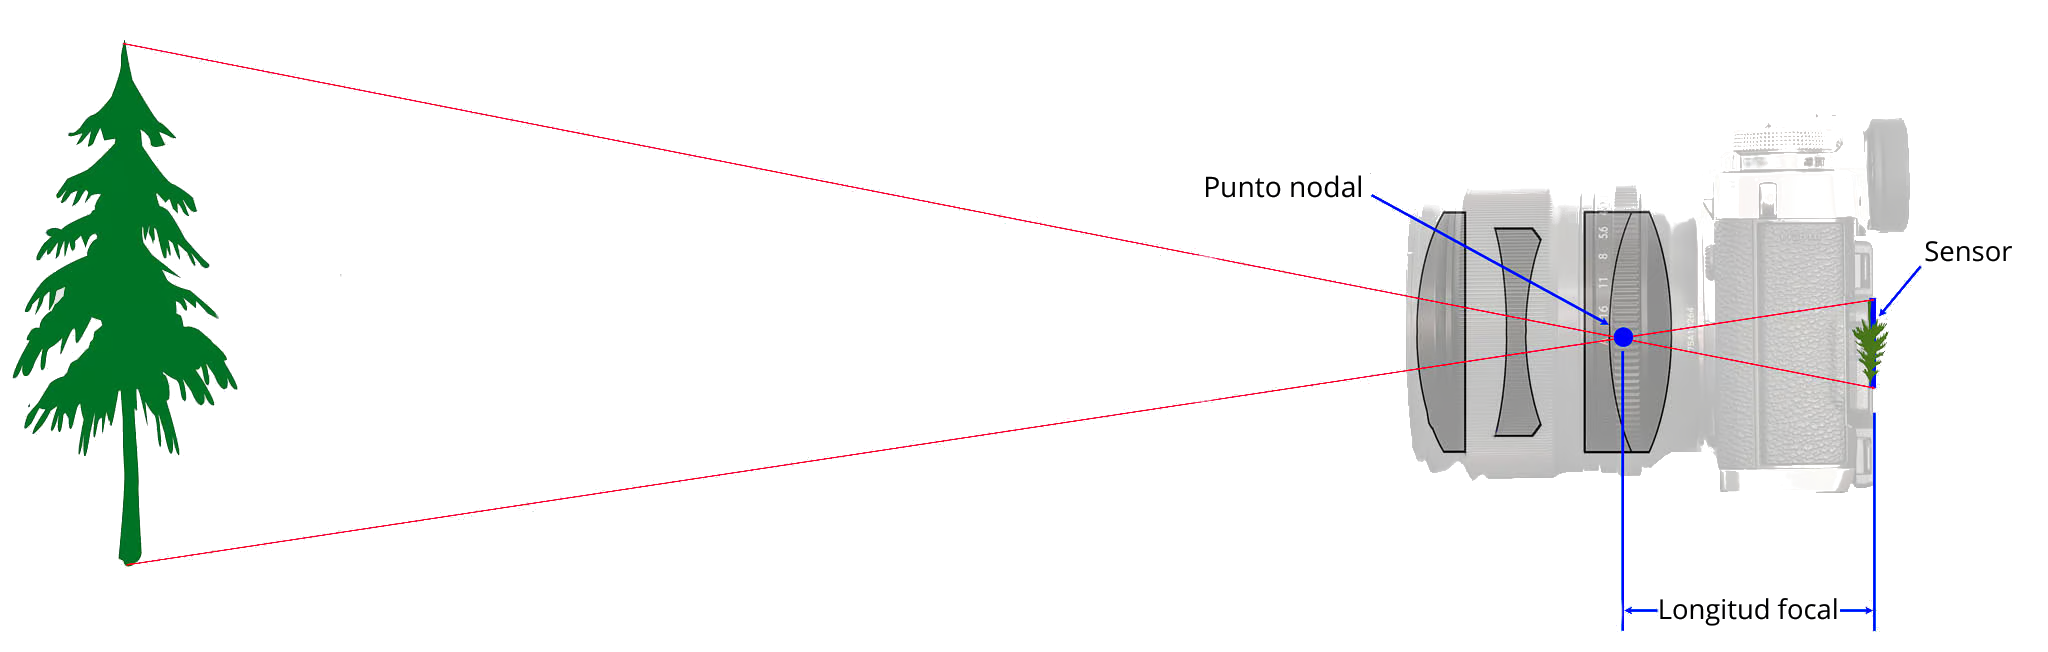
\includegraphics[scale=0.2]{imagenes/cap2/focal.png}
	\caption[Relación entre punto nodal y longitud focal.]{Relación entre punto nodal y longitud focal \cite{44}}
	\label{fig11}
\end{figure}

La longitud focal es un factor importante, ya que determina el campo de visión de una lente, es decir, la cantidad de escena que se captura (ver Figura \ref{fig11.2}).  En longitudes focales más largas, los objetos parecen estar más cerca del objetivo de la cámara, lo que puede hacer que parezcan más grandes en la imagen. Por el contrario, con longitudes focales más cortas, los objetos aparentan estar más distantes en la fotografía.

\begin{figure}[h]
	\centering
	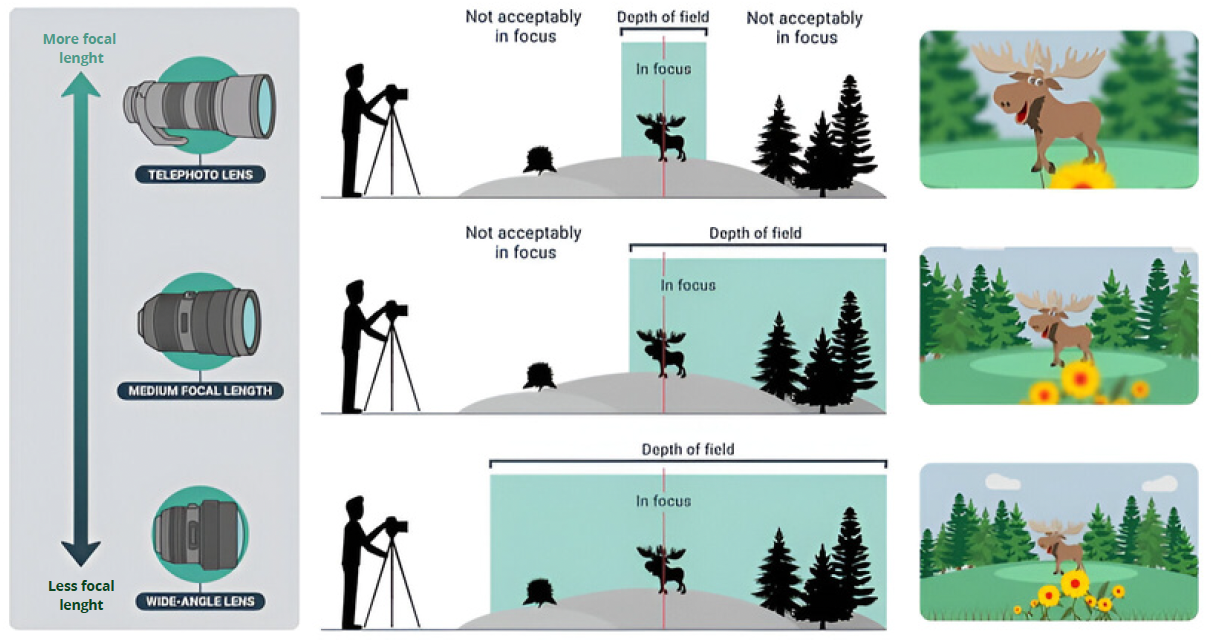
\includegraphics[scale=0.55]{imagenes/cap1/perspective.png}
	\caption[Relación entre longitud focal y campo de visión.]{Relación entre longitud focal y campo de visión. La longitud focal afecta al tamaño aparente de los objetos y a la cantidad de escena que aparece en la imagen.}
	\label{fig11.2}
\end{figure}

\subsection*{Sensor de la cámara}
El sensor de la cámara es el componente encargado de capturar la luz y transformarla en una imagen digital. Su tamaño incide directamente en la calidad de la imagen y en su capacidad para capturar la luz. El estándar comúnmente utilizado es de 36mm x 24mm, conocido como \textit{full frame} o 35mm, siendo este tamaño una referencia debido a su similitud con el formato de película fotográfica analógica utilizado en el pasado.

La necesidad de establecer un estándar es esencial para comparar equitativamente imágenes capturadas por diferentes dispositivos. Al referirnos a un estándar de 35 mm, disponemos de un sistema de referencia común que nos permite convertir las imágenes, de manera que los objetos visibles en la escena tengan dimensiones similares, facilitando así su comparación y análisis.

Otra manera de expresar el tamaño del sensor es a través del factor de recorte, que se calcula como la proporción entre el tamaño del sensor de 35 mm y el de nuestra cámara (ver Figura \ref{fig12}). El factor de recorte se emplea a menudo para comprender la dimensión del sensor de la cámara en relación con el estándar de 35 mm. Esta medida facilita una comparación directa entre el tamaño del sensor de 35 mm y el de nuestra cámara, lo que permite entender mejor su capacidad para capturar imágenes.

\begin{figure}[h]
	\centering
	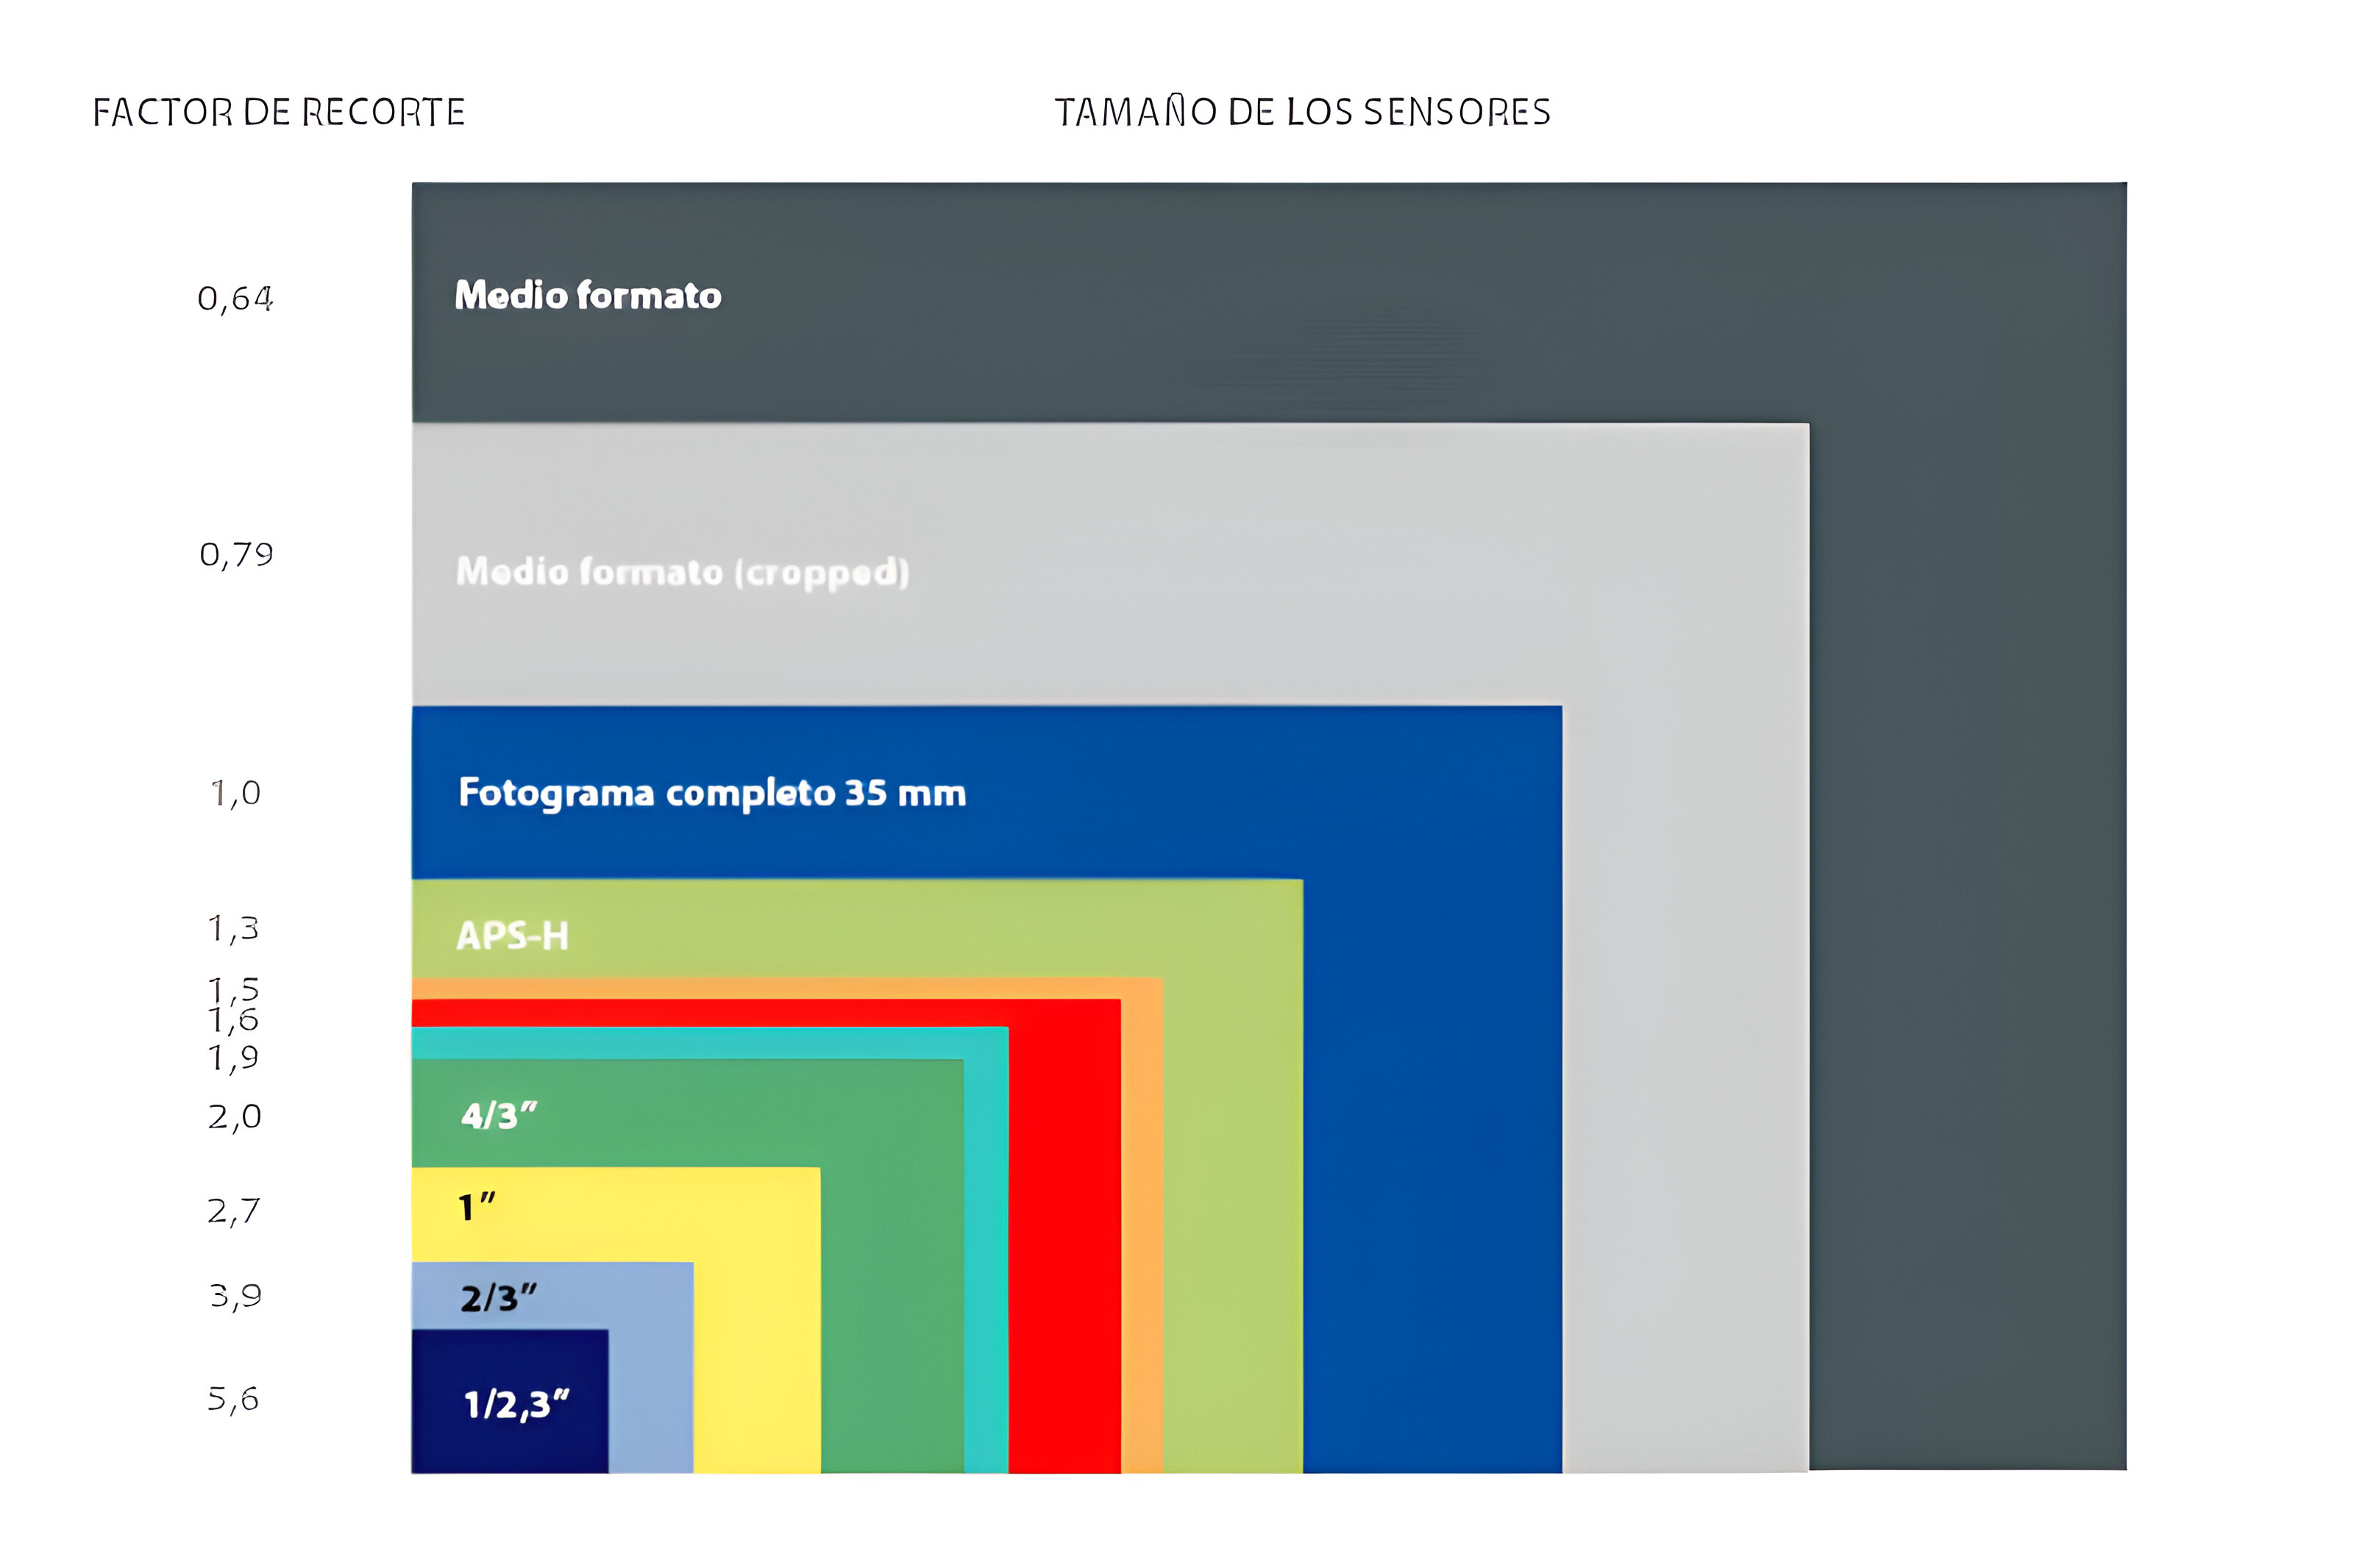
\includegraphics[scale=0.08]{imagenes/cap2/tam_sensor_factor.jpeg}
	\caption[Tipos de tamaños de sensor.]{Tamaños del sensor expresados según el factor de recorte \cite{48}}
	\label{fig12}
\end{figure}

Uno de los aspectos más importantes del factor de recorte es su impacto en la longitud focal, lo que nos lleva al concepto de \textit{longitud focal equivalente}. Por ejemplo, al tener una focal de 300 mm en un sensor con factor de recorte 1.6, estaríamos obteniendo un efecto equivalente al de una focal de 480 mm (300 mm x 1.6) en un sensor \textit{full frame} con factor de recorte 1.

\begin{figure}[h]
	\centering
	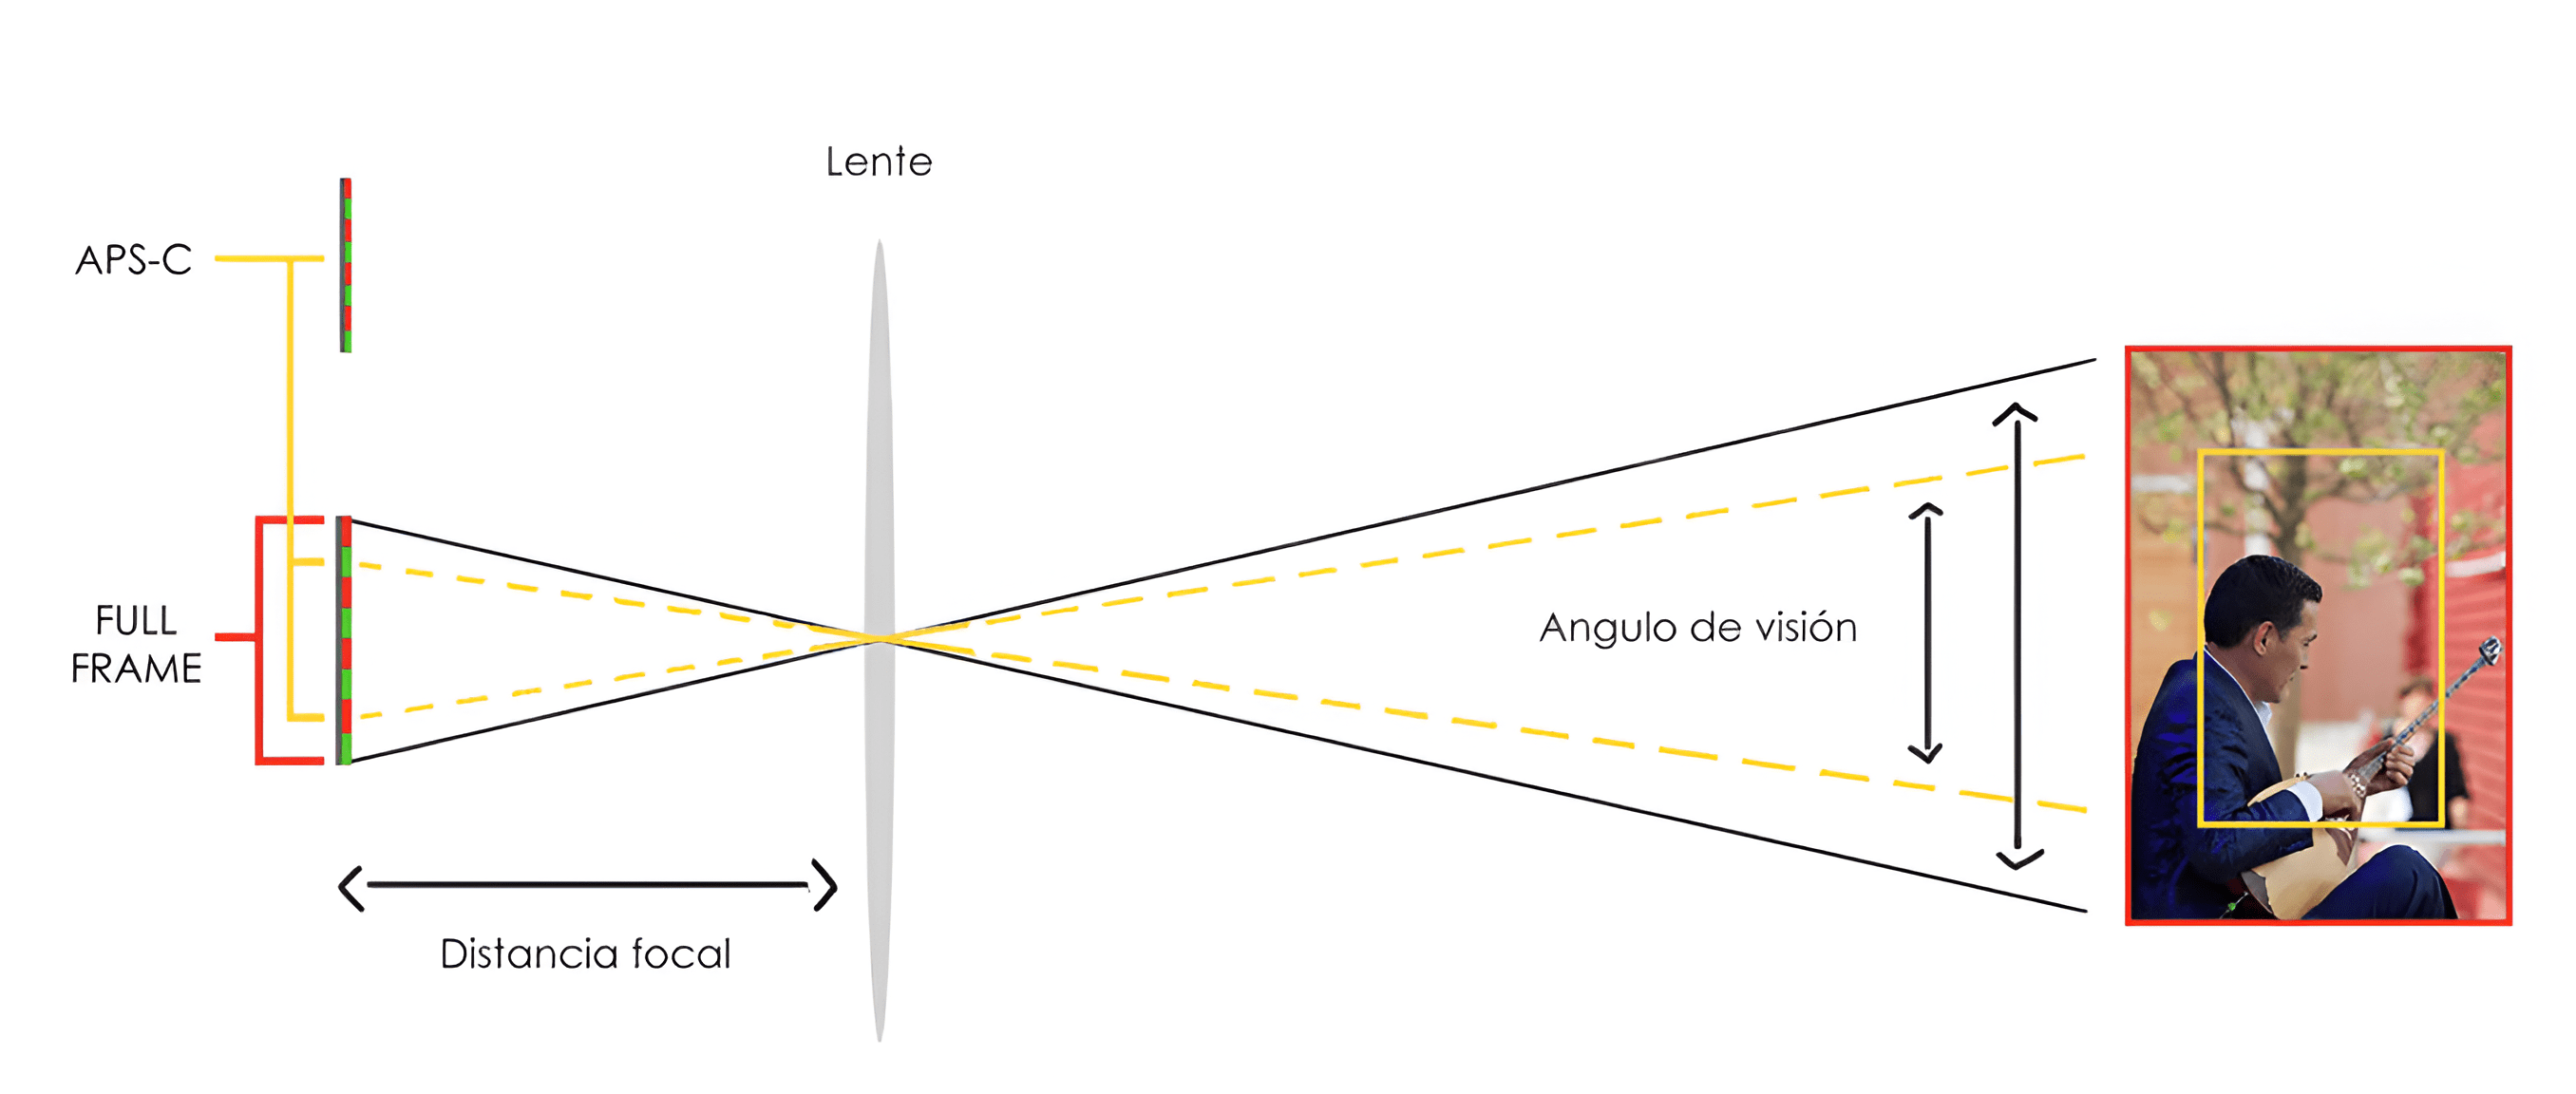
\includegraphics[scale=0.13]{imagenes/cap2/focal-equivalente.png}
	\caption[Ejemplo de longitud focal equivalente.]{Ejemplo de longitud focal equivalente según el tamaño del sensor \cite{46}.}
	\label{fig13}
\end{figure}


\subsection*{Distancia cámara-sujeto}

La distancia cámara-sujeto se define como la separación física entre la cámara y el sujeto que está siendo fotografiado (ver Figura \ref{fig14}). Modificar esta distancia provoca variaciones en la apariencia visual del rostro en la fotografía obtenida \cite{43}. Este fenómeno se conoce como distorsión de perspectiva.

\begin{figure}[h]
	\centering
	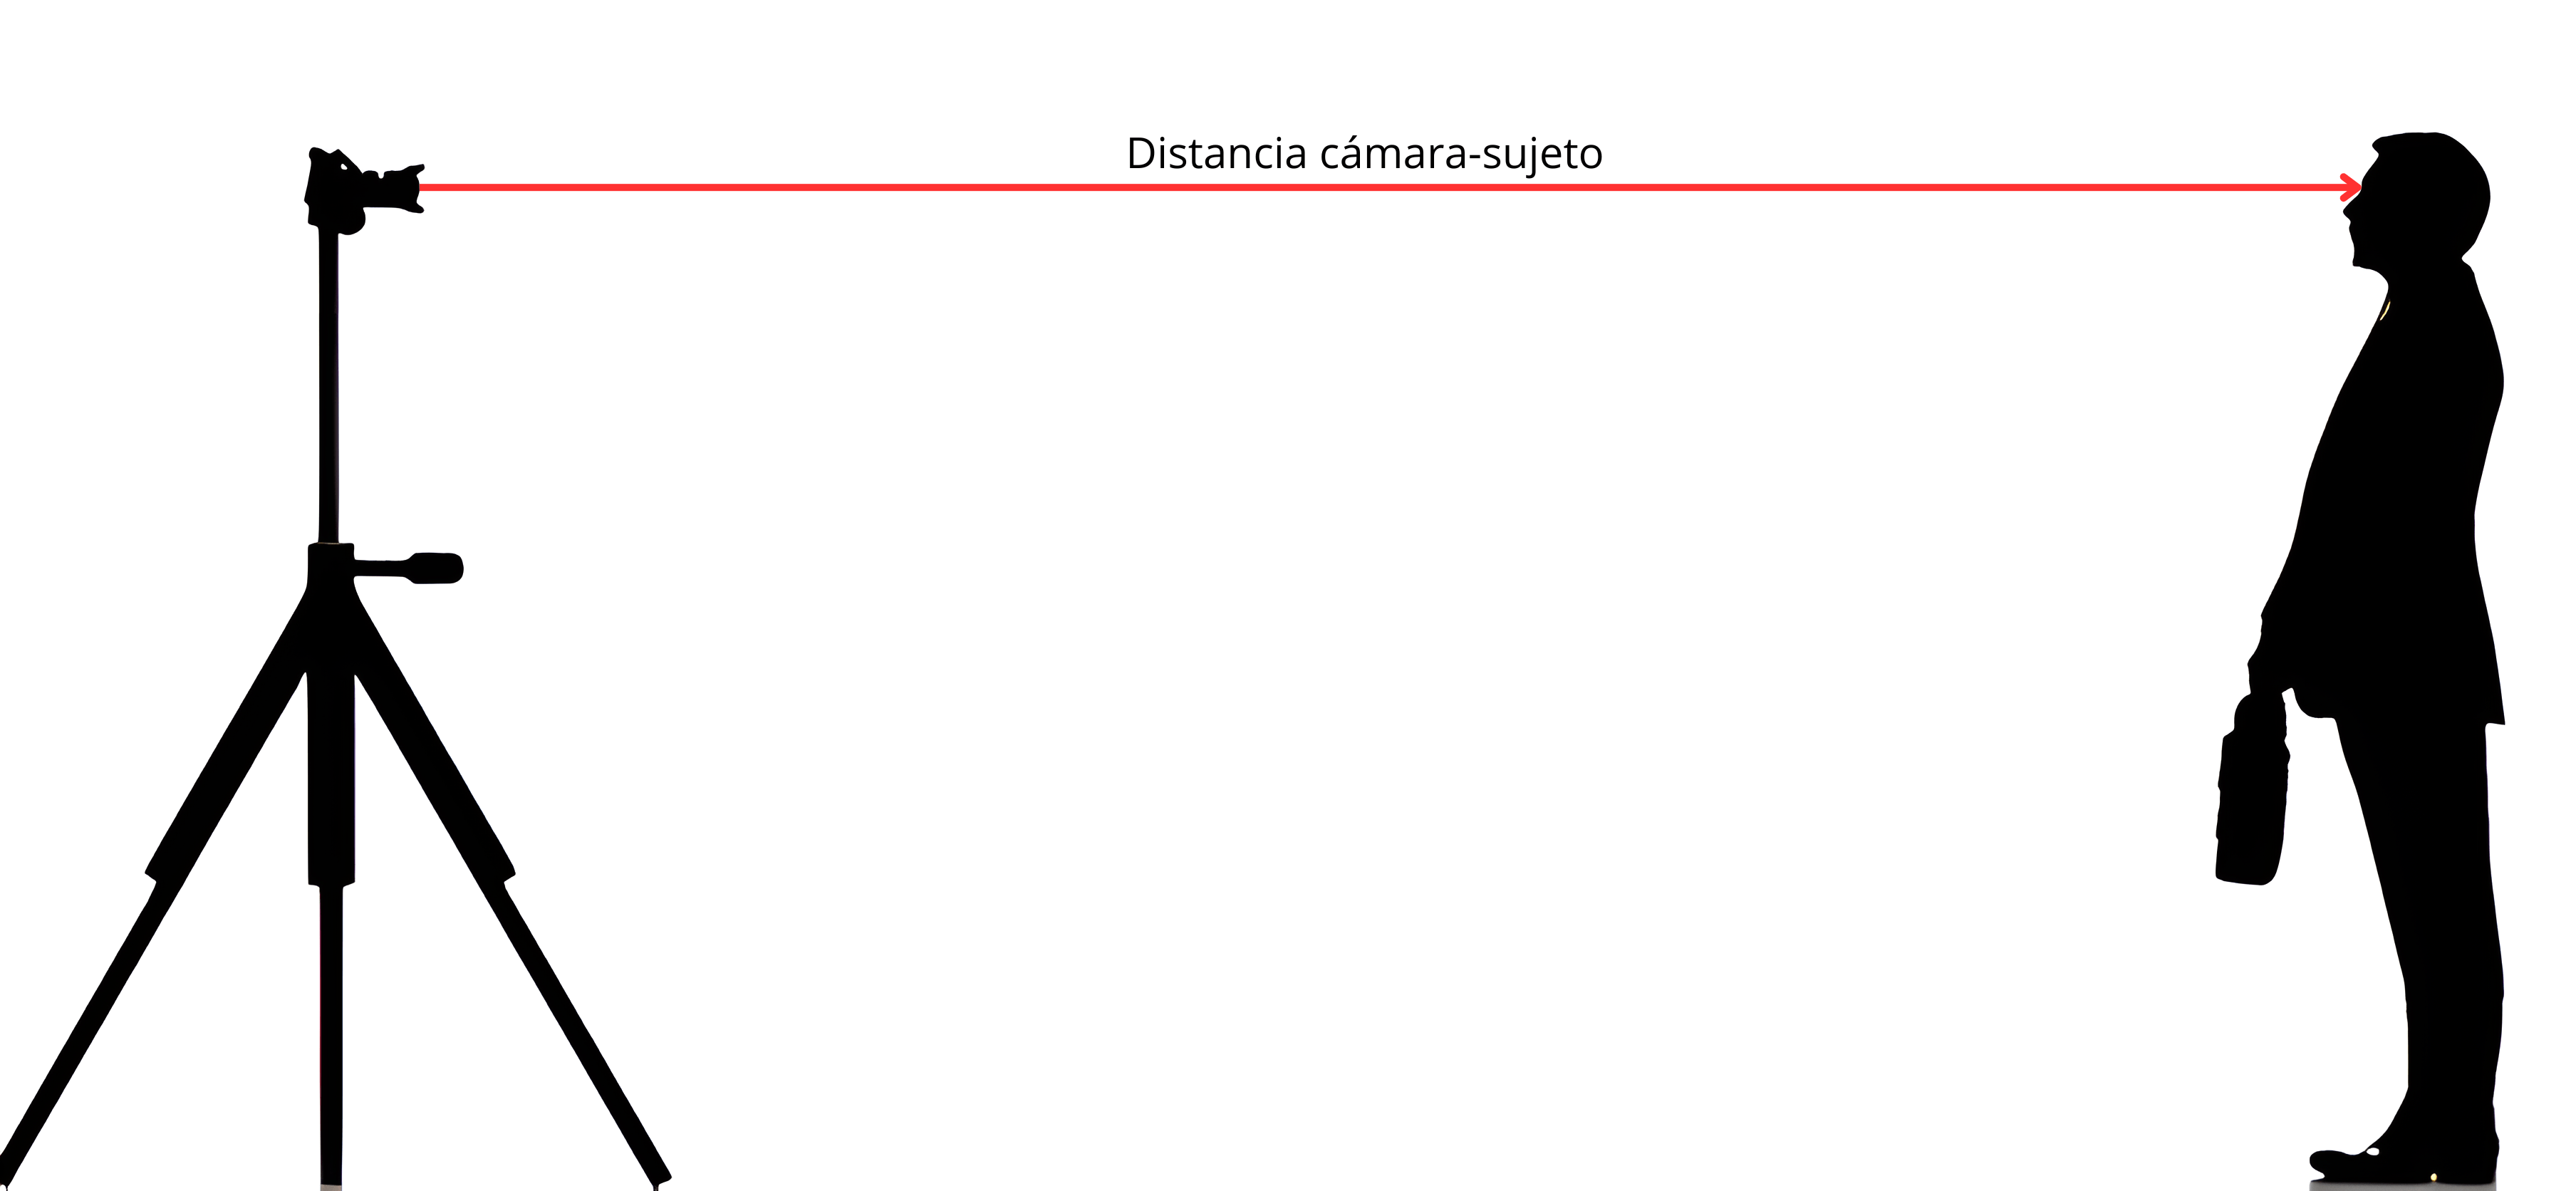
\includegraphics[scale=0.1]{imagenes/cap2/SCD_final.png}
	\caption[Distancia desde la cámara al sujeto.]{Distancia desde la cámara al sujeto.}
	\label{fig14}
\end{figure}

La distorsión de perspectiva \cite{8,51} es la transformación que sufre un objeto y su entorno debido a la proximidad del mismo respecto al objetivo (ver Figura \ref{fig15}). En el caso de las fotografías faciales, cuanto menor es la distancia cámara-sujeto, mayor es la distorsión de perspectiva que afecta a la persona fotografiada. Esto afecta a rasgos de la cara que pueden aparecer más grandes, como la nariz, o más pequeños, como las orejas, de lo que realmente son (ver Figura \ref{fig2}).

\begin{figure}[h]
	\centering
	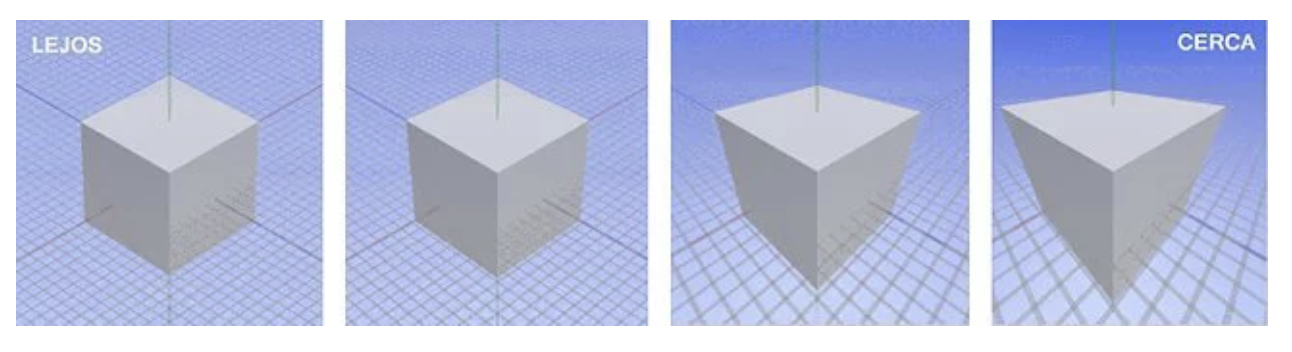
\includegraphics[scale=0.5]{imagenes/cap2/distorsion.png}
	\caption[Efectos de la distorsión según distancia.]{Efecto de la distorsión conforme se acerca la cámara al objeto \cite{51}.}
	\label{fig15}
\end{figure}

Uno de los malentendidos comunes en fotografía es la creencia de que la longitud focal distorsiona los rasgos faciales, sin embargo, la longitud focal no tiene nada que ver con la distorsión del rostro de un sujeto, siendo esta únicamente provocada por la distancia de la cámara al sujeto \cite{52}.



